%% article.tex -- versão em PORTUGUÊS do artigo submetido ao IEEE/IFIP NOMS.
%%
%% Grafos de Conhecimento Centrados na Sessão HTTP para Detecção Explicável
%% e Mitigação de Escopo Derivado de DDoS de Camada de Aplicação
%%
%% Tradução fiel de papers/http-session-noms/article.tex, mesmo conteúdo e mesmos
%% números. Mantém o formato IEEEtran de duas colunas.
%%
%% NOTA SOBRE PAGINAÇÃO: o limite de 8 páginas de corpo vale para a submissão ao
%% NOMS, que é em inglês. Esta versão não está sujeita a ele — o português corre
%% 15-20% mais longo que o inglês, e comprimir para caber custaria conteúdo sem
%% ganho nenhum. Use a versão em inglês para submeter.

\documentclass[conference,letterpaper,10pt]{IEEEtran}
\IEEEoverridecommandlockouts

\usepackage[T1]{fontenc}
\usepackage[utf8]{inputenc}
\usepackage[brazilian]{babel}
%% O babel troca \figurename para "Figura", mas as chamadas no texto usam
%% "Fig." como no original. Fixa os dois no formato do IEEEtran.
\addto\captionsbrazilian{\renewcommand{\figurename}{Fig.}}
\usepackage{cite}
\usepackage{amsmath,amssymb}
\usepackage{graphicx}
\usepackage{booktabs}
\usepackage{algorithm}
\usepackage{algorithmic}
\usepackage{url}
\usepackage[hidelinks]{hyperref}

%% Ver comentario equivalente na versao em ingles.
\setlength{\textfloatsep}{10pt plus 2pt minus 2pt}
\setlength{\intextsep}{8pt plus 2pt minus 2pt}
\setlength{\dbltextfloatsep}{10pt plus 2pt minus 2pt}

%% Contador proprio para os blocos de codigo: como floats \begin{figure} eles
%% abriam buracos na numeracao das figuras-imagem. O estilo ieeelst reproduz a
%% legenda "Fig. N. Texto" do IEEEtran.
\usepackage{float}
\makeatletter
\newcommand\floatc@ieeelst[2]{\setbox\@tempboxa\hbox{\footnotesize #1.\enskip #2}%
  \ifdim\wd\@tempboxa>\hsize \footnotesize #1.\enskip #2\par
  \else \hbox to\hsize{\hfil\box\@tempboxa\hfil}\fi}
\newcommand\fs@ieeelst{\def\@fs@cfont{\footnotesize}\let\@fs@capt\floatc@ieeelst
  \def\@fs@pre{}\def\@fs@mid{\vspace\abovecaptionskip}\def\@fs@post{}%
  \let\@fs@iftopcapt\iffalse}
\makeatother
\floatstyle{ieeelst}
\newfloat{listing}{tbp}{lol}
\floatname{listing}{Listagem}

%% O IEEEtran usa URW Courier (pcr) para \texttt. Onde essas metricas nao
%% existem, cai para Latin Modern Mono -- e NAO para cmtt: sem o cm-super
%% instalado, cmtt em T1 gera bitmaps Type 3, que o IEEE PDF eXpress sinaliza
%% e que ficam serrilhados na tela. lmtt e Type 1 e ja vem no TeX Live.
\IfFileExists{pcrr8t.tfm}{}{\renewcommand{\ttdefault}{lmtt}}

\begin{document}

\title{Grafos de Conhecimento Centrados na Sessão HTTP para Detecção Explicável\\
e Mitigação de Escopo Derivado de DDoS de Camada de Aplicação}

\author{\IEEEauthorblockN{Natanael Oliveira, Arthur Kobielski e Marcos Luna}
\IEEEauthorblockA{Instituto de Informática, Universidade Federal do Rio Grande do Sul (UFRGS), Porto Alegre, Brasil\\
\{natanael.oliveira, arthur.kobielski, marcos.luna\}@inf.ufrgs.br}}

\maketitle

\begin{abstract}
Campanhas distribuídas de Slow HTTP DoS mantêm cada origem abaixo de qualquer
limiar razoável por sessão, de modo que o sinal de ataque mora na estrutura
\emph{entre} sessões e não dentro de nenhuma delas. Os detectores descartam essa
estrutura ao reduzir a sessão a um vetor numérico, e os detectores recentes
baseados em grafos de conhecimento raciocinam em nível de nó de rede e param no
relatório textual. Modelamos a sessão HTTP como entidade ontológica de primeira
classe em OWL e substituímos a relação plana \texttt{relatedTo} por seis
sub-propriedades tipadas, ponderadas pelo custo que o atacante teria para quebrar
cada sinal; a proximidade de rede fica em último lugar porque \emph{botnets}
modernas se distribuem agressivamente entre ASNs e prefixos. Uma regra SPARQL/SWRL
dispara sobre a massa ponderada dessas sub-relações, e sua derivação \emph{é} o
veredicto, exportado como cadeia de evidência em JSON-LD e STIX~2.1 cujo
discriminador define o escopo da mitigação. Contra campanhas furtivas
distribuídas, a detecção por sessão permanece no acaso em quatro famílias de
modelo, mesmo com o conjunto completo de atributos de fluxo, enquanto o raciocínio
entre sessões as detecta de forma consistente (ROC AUC $0{,}50$ \emph{vs.}\
$0{,}98$; $d = 22{,}4$). Em \emph{datasets} públicos, cujos ataques carregam
assinatura de fluxo evidente, um \emph{baseline} por sessão forte já basta, e
reportamos essa delimitação explicitamente. Mostramos ainda que a maneira óbvia
de derivar o escopo da mitigação é nociva: a propriedade que a maioria do
\emph{cluster} compartilha é um \emph{fingerprint} \emph{legítimo} assim que a
\emph{botnet} abrange vários \emph{stacks} TLS, bloqueando $0\%$ do ataque e
$39\%$ dos usuários. Escolher o discriminador por enriquecimento sobre um perfil
de tráfego normal bloqueia $85$--$90\%$ a $0{,}00\%$ de colateral. E, avaliado
como detector, esse caminho simbólico dispensa treino e limiar, recuperando de
duas a cinco vezes mais de uma campanha fragmentada do que o modelo aprendido
consegue no mesmo ponto de operação de falso positivo zero.
\end{abstract}

\begin{IEEEkeywords}
gestão de segurança, grafo de conhecimento, DDoS de camada de aplicação, modelos
semânticos, raciocínio automatizado, explicabilidade, política de mitigação
\end{IEEEkeywords}

%% ====================================================================
\section{Introdução}
\label{sec:intro}

O DDoS de camada de aplicação mudou de natureza, não apenas de escala. Em agosto
de 2023, o HTTP/2 Rapid Reset (CVE-2023-44487) levou os picos mitigados a 398
milhões de requisições por segundo, a partir de uma \emph{botnet} de cerca de
vinte mil máquinas~\cite{cve202344487,google2023rapidreset}, e a Cloudflare
bloqueou mais de 6\,500 ataques hiper-volumétricos só no segundo trimestre de
2025, com o DDoS sobre HTTP crescendo 129\% ano a
ano~\cite{cloudflare2025q2ddos}. As defesas volumétricas respondem pela ponta
ruidosa desse espectro. A ponta silenciosa é mais difícil. A família de ataques
\emph{distribuídos de Slow HTTP DoS} abrange o Slowloris e seus descendentes,
mais variantes baseadas em taxa que ainda sustentam conexões abertas, como HULK e
GoldenEye~\cite{cambiaso2013slowdos}. Esses ataques exaurem um servidor a partir
de muitas origens coordenadas, cada uma contribuindo tão pouco que nenhum limiar
por origem é ultrapassado. Ataques modernos sobre HTTP/2 compartilham essa
propriedade de exaustão multi-origem, mas operam por mecanismos distintos,
notadamente cancelamento de \emph{stream} e abuso de cabeçalhos de continuação.
Esses exigem sub-relações fora do escopo que avaliamos aqui, e os tratamos como
alvo de extensão imediata (Seção~\ref{sec:conclusion}), não como afirmação deste
artigo.

Vista isoladamente, cada requisição é indistinguível de uma legítima. O sinal
mora na estrutura \emph{entre} sessões: duração da conexão, entropia de rotas,
consistência do \emph{fingerprint} do cliente e a convergência de muitas origens
num mesmo \emph{endpoint} sob uma mesma assinatura de
cliente~\cite{kemp2023approach}.

Isto é tanto um problema de gestão de redes e serviços quanto de detecção. Um
operador não precisa de um rótulo; precisa saber \emph{quais} clientes bloquear,
com base em \emph{qual} evidência, e com um filtro estreito o bastante para não
desconectar os usuários legítimos do próprio serviço sob ataque.

A literatura reconhece a primeira metade e ignora largamente a segunda. A
meta-análise de Odusami et al.~\cite{odusami2020survey}, sobre setenta e cinco
estudos, mostra que 47\% dos métodos de DDoS de camada de aplicação derivam
atributos de sessões, como taxa de requisições por usuário, duração média e
operações por identidade. Em todos eles a sessão é achatada num vetor numérico
antes de chegar ao classificador. O detector vê estatísticas, não sessões, e por
isso não consegue raciocinar sobre identidades reaproveitadas, sobre
\emph{fingerprints} convergindo num \emph{endpoint}, ou sobre padrões que só
existem entre duas sessões individualmente normais.

Trabalhos contemporâneos atacam a opacidade desses detectores com grafos. O
KLAGE, de Belcastro et al.~\cite{belcastro2025klage}, constrói grafos de
conhecimento a partir de \emph{logs} de rede, classifica nós com Graph-BERT e
produz relatórios em linguagem natural via LIME e modelos de linguagem grandes,
atingindo $F_1 = 84{,}1\%$ em \emph{benchmarks} IoT que incluem DDoS Slowloris. É
evidência sólida de que grafos de conhecimento são substrato viável de detecção
em tempo de execução. Três lacunas, contudo, permanecem. Sua
unidade de raciocínio é o \emph{nó de rede} (porta, IP, fluxo), e não a sessão de
aplicação. A coordenação é capturada implicitamente em \emph{embeddings}
aprendidos, e não em relações simbólicas nomeadas. E o \emph{pipeline} termina num
relatório, sem uma política de mitigação cujo escopo derive do próprio grafo.
Essas três lacunas delimitam o espaço que este artigo ocupa.

\textbf{Contribuições.} São quatro:

\begin{enumerate}
\item \textbf{A sessão HTTP como entidade ontológica de primeira classe, com uma
família \texttt{relatedTo} ponderada.} Uma ontologia OWL modela
\texttt{ApplicationSession} com relações tipadas para identidade do cliente,
\emph{endpoint} alvo, comportamento exibido e mitigação aplicável, e substitui a
relação plana \texttt{relatedTo} por uma família de \emph{seis sub-propriedades
tipadas e ponderadas}. Os pesos codificam o custo que o atacante teria para
quebrar cada sinal. A proximidade de rede, trivialmente quebrada por
\emph{botnets} modernas, entra portanto como evidência auxiliar e nunca como
pré-requisito.

\item \textbf{Raciocínio simbólico sobre a soma ponderada das sub-relações.} Um
\emph{pipeline} em tempo de execução eleva eventos HTTP a instâncias da ontologia,
instanciando cada sub-propriedade independentemente a partir de sua própria
evidência. Uma regra SPARQL/SWRL dispara sobre a massa ponderada de coordenação
$\Omega(S)$ de um \emph{cluster} candidato. O veredicto é a derivação que
satisfez a regra, não a saída de um classificador interpretada a posteriori.

\item \textbf{Uma cadeia de evidência acoplada à derivação automática de escopo de
mitigação.} Cada veredicto carrega uma cadeia em JSON-LD e STIX~2.1 que lista as
sub-relações ativadas, seus pesos e os valores que satisfizeram a regra, e o
escopo da mitigação é derivado do mesmo grafo. Mostramos que a maneira natural de
derivá-lo, pela propriedade que a maioria do \emph{cluster} compartilha, é
ativamente nociva em condições realistas, e a substituímos por um critério
baseado em enriquecimento sobre um perfil de tráfego normal.

\item \textbf{Uma avaliação parametrizada pelo grau de distribuição, com métrica
de dano colateral.} Contra um \emph{baseline} por sessão deliberadamente
\emph{forte}, a ablação isola o ganho do raciocínio entre sessões e o ganho
específico dos sinais de peso alto sobre a proximidade de rede. Reportamos também
a fração de tráfego legítimo atingida pela mitigação resultante, métrica
auto-reportada por produtos comerciais de \emph{bot management} mas, até onde
sabemos, não usada sistematicamente na literatura acadêmica de Camada 7. A
implementação de referência é código aberto.
\end{enumerate}

A Seção~\ref{sec:related} posiciona o trabalho, a Seção~\ref{sec:approach}
apresenta o arcabouço, as Seções~\ref{sec:method} e~\ref{sec:results} a
metodologia e os resultados, e a Seção~\ref{sec:discussion} as limitações que
delimitam a afirmação.

%% ====================================================================
\section{Trabalhos Relacionados}
\label{sec:related}

\subsection{Grafos de Conhecimento em Segurança e Gestão}

A primeira onda de grafos de conhecimento em segurança foi \emph{estática}:
entidades extraídas de CVEs, relatórios e \emph{blogs}, normalizadas e ligadas
numa base consultável~\cite{jia2018practical,bonagiri2024practical}. O
levantamento de Liu et al.~\cite{liu2022recent} enuncia a lacuna resultante sem
rodeios: ``ainda é pouco claro como implementar o grafo de conhecimento para
enfrentar dificuldades industriais reais em situações de ataque e defesa
cibernética''. Grafos construídos a partir de texto de inteligência de ameaças não
capturam estrutura de tráfego em tempo de execução.

Trabalhos mais recentes populam grafos a partir do próprio tráfego. O
KLAGE~\cite{belcastro2025klage} é o exemplar mais próximo e aquele contra o qual
comparamos. Representações em grafo também vêm ganhando espaço em tarefas de
gestão adjacentes à nossa: Sadlek et al.~\cite{sadlek2024device} identificam
dependências entre dispositivos por predição de arestas sobre grafos de rede, e
Wang e Stadler~\cite{wang2024intrusion} aprendem sequências de ações de ataque a
partir de medições em \emph{testbed}. Ambos operam sobre entidades em nível de
rede. Diferimos deles em três eixos. Nossa unidade de raciocínio é a sessão de
aplicação; nosso formalismo são relações simbólicas nomeadas, e não
\emph{embeddings} aprendidos; e nossa saída inclui o escopo da mitigação.

\subsection{Detecção de DDoS de Camada 7 sobre HTTP}

A detecção se organiza historicamente em duas famílias, sobre um corpo de
levantamentos que consolidam o domínio~\cite{tripathi2021application,cambiaso2013slowdos}. O perfilamento estatístico
constrói linhas de base a partir de estatísticas agregadas de fluxo ou sessão:
Fernandes et al.~\cite{fernandes2015autonomous} com PCA sobre estatísticas de
fluxo, e Bharathi e Sukanesh~\cite{bharathi2012pca} com PCA sobre uma matriz
comportamental por sessão, que é uma das primeiras formulações a colocar a sessão
no centro, ainda que como vetor de atributos. O aprendizado supervisionado sobre
atributos de sessão é a segunda família, com Kemp et al.~\cite{kemp2023approach}
como representante mais recente; seus autores registram que o método não foi
validado em tempo real e que a saída é binária, sem explicação ontológica. O denominador
comum é que a sessão é tratada como agregado de atributos, nunca como entidade
sobre a qual se possa raciocinar.

\subsection{Modelagem de Sessão em Detecção de Anomalias}

A meta-análise de Odusami et al.~\cite{odusami2020survey} fornece a evidência
quantitativa mais clara sobre como a sessão é tratada: em 47\% dos métodos
catalogados, atributos derivados de sessão alimentam o classificador, mas em
nenhum dos setenta e cinco estudos a sessão é mantida como objeto com identidade,
alvo, comportamento e relações tipadas. A redução é uniforme, e é ela que coloca
fora do alcance do detector o raciocínio sobre identidades reaproveitadas, sobre
\emph{fingerprints} convergindo num \emph{endpoint}, ou sobre padrões visíveis
apenas entre sessões.

Plataformas industriais de \emph{bot management} de fato exploram estrutura entre
sessões, agrupando sessões aparentemente independentes por similaridade de
\emph{stack} TLS através de \emph{fingerprints} da família
JA4~\cite{althouse2023ja4}. São, contudo, proprietárias, sem ontologia pública,
sem \emph{benchmark} acadêmico reprodutível e sem métrica formalizada de dano
colateral. Formalizar essa prática de modo auditável, e derivar o escopo de
mitigação de uma regra ontológica explícita, é o que permanece em aberto.

%% ====================================================================
\section{Grafo de Conhecimento Centrado na Sessão}
\label{sec:approach}

\begin{figure*}[t]
\centering
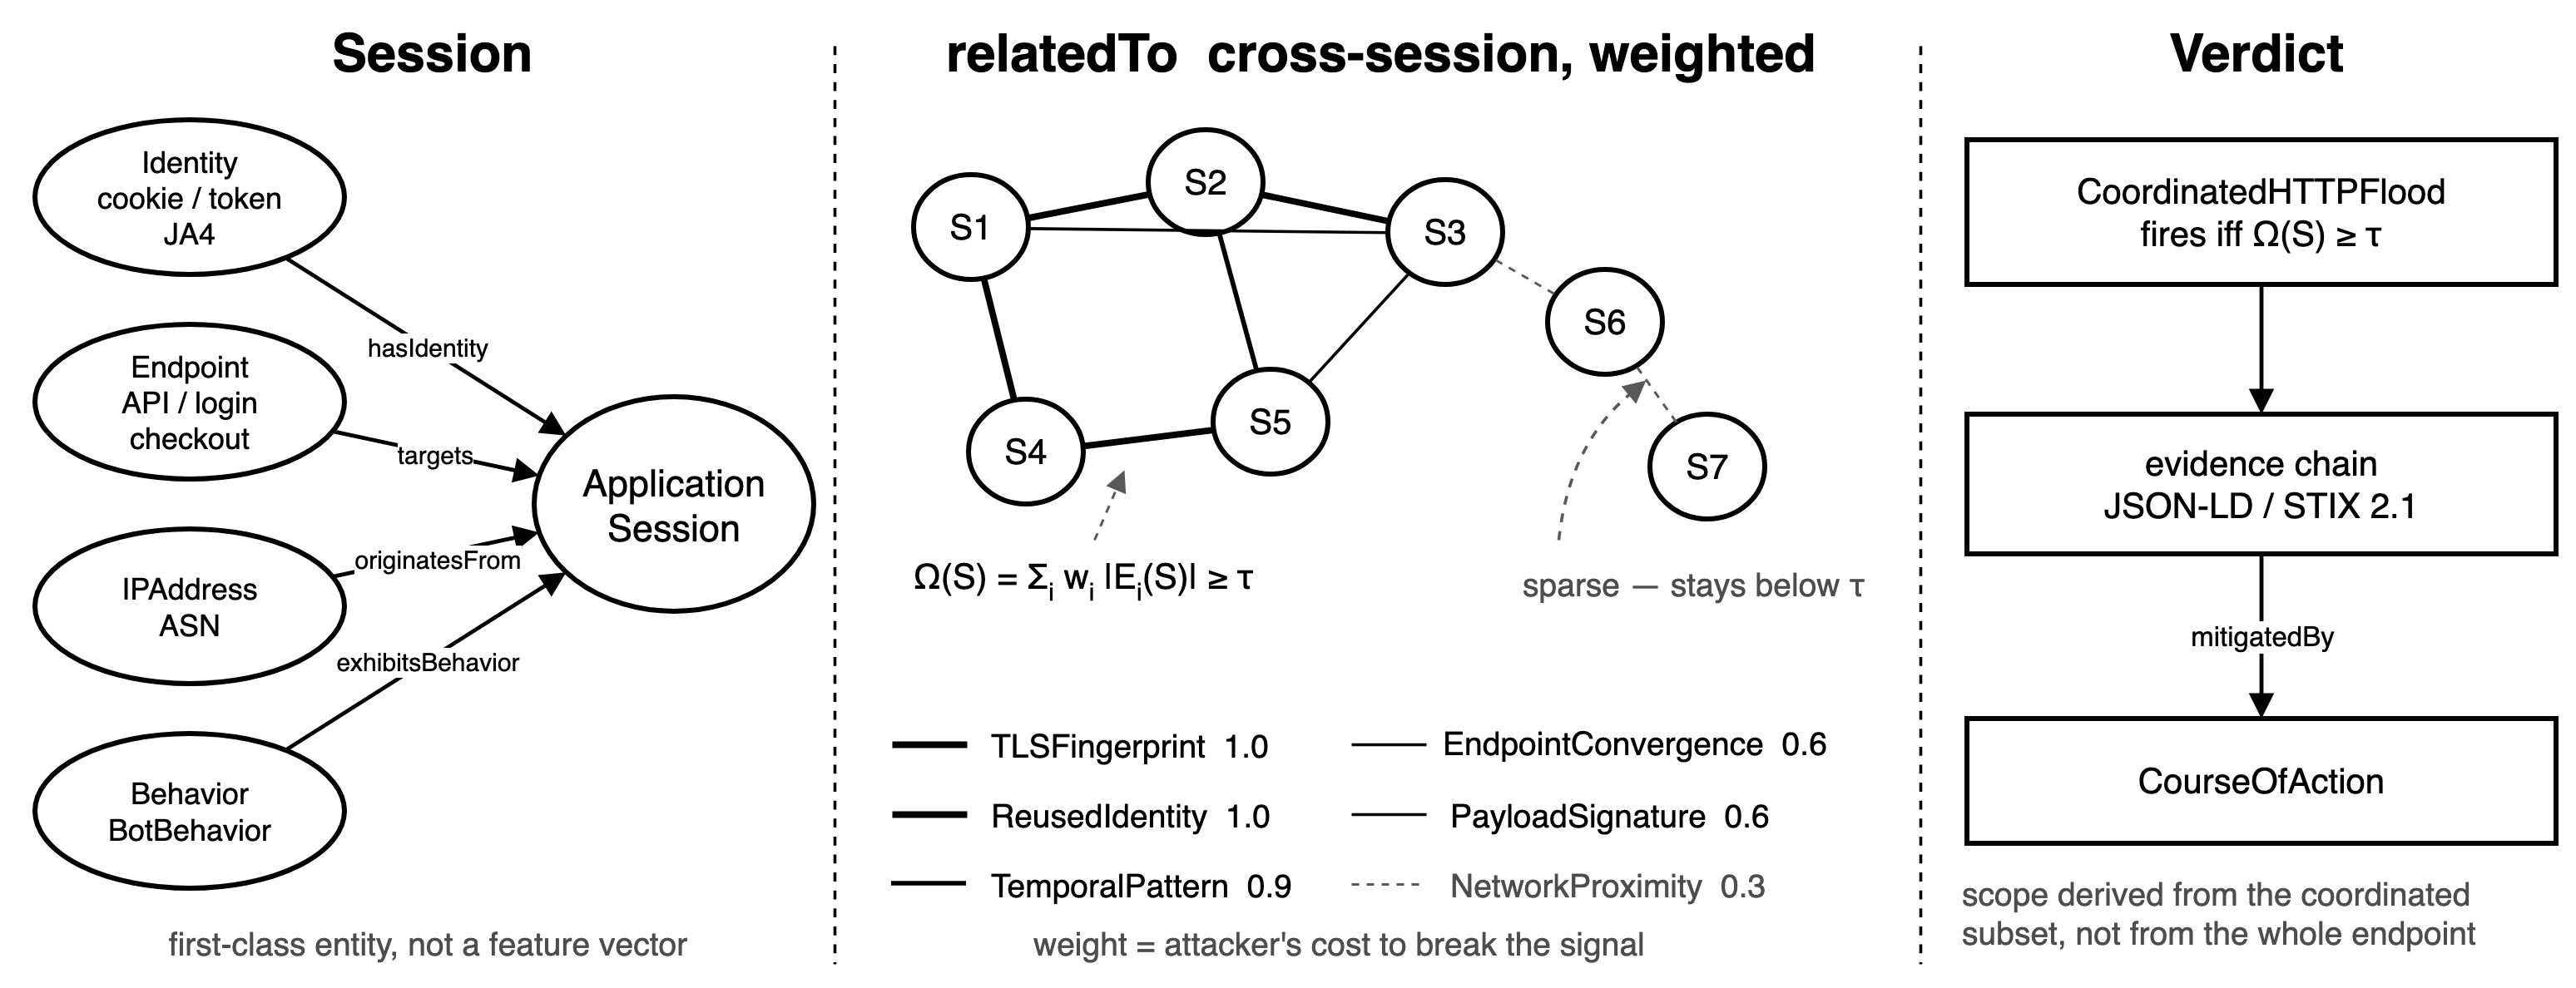
\includegraphics[width=\textwidth]{figures/fig1_ontology.png}
\caption{Ontologia centrada na sessão. \texttt{ApplicationSession} é entidade de
primeira classe, com relações primárias tipadas para identidade, origem,
\emph{endpoint} e comportamento; a família \texttt{relatedTo} ponderada liga as
sessões entre si; e a regra de detecção acopla o veredicto simbólico a um curso de
ação cujo escopo é derivado do subconjunto coordenado.}
\label{fig:ontology}
\end{figure*}

A Fig.~\ref{fig:ontology} resume o arcabouço. Quatro estágios operam sobre o
tráfego ao vivo: eventos HTTP são ingeridos; elevados a instâncias da ontologia,
com sessões como nós persistentes do grafo; avaliados por regras semânticas; e
convertidos num veredicto que carrega sua cadeia de evidência e o escopo de
mitigação derivado.

\subsection{Ontologia}
\label{sec:ontology}

A classe central é \texttt{ApplicationSession}, ligada por \texttt{hasIdentity} a
uma \texttt{Identity} composta (\emph{cookie}, \emph{token} JWT, \emph{username},
\emph{fingerprint} TLS), por \texttt{targets} a um \texttt{Endpoint}
(\texttt{AuthEndpoint}, \texttt{APIEndpoint}, \texttt{StaticAsset}), por
\texttt{exhibitsBehavior} a um perfil comportamental, e por \texttt{mitigatedBy} a
uma política (\texttt{RateLimit}, \texttt{Challenge}, \texttt{Block}) que carrega
um atributo \texttt{scope}. A classe abstrata \texttt{ApplicationLayerAttack} se
especializa em \texttt{SlowHTTPDoSFamily}, por sua vez dividida em
\texttt{ConnectionExhaustionAttack} (Slowloris, \emph{slow body}, \emph{slow
read}) e \texttt{CoordinatedHTTPFlood} (HULK, GoldenEye). A ontologia está
alinhada a STIX~2.1~\cite{oasis2021stix} e MITRE ATT\&CK, e declara também
\texttt{CredentialStuffing} e \texttt{CoordinatedAPIAbuse}, que reaproveitam a
mesma maquinaria mas estão fora do escopo experimental deste artigo.

\subsection{Modelo de Ameaça}
\label{sec:threat}

O defensor opera a aplicação atacada e observa, por requisição, o
\emph{ClientHello} TLS (e portanto um \emph{fingerprint} JA4), endereço de origem
e prefixo/ASN, \emph{endpoint} alvo, instante de chegada, e o material de
identidade que a aplicação expuser. Ele não observa o canal de controle da
\emph{botnet} e não tem verdade de campo sobre quais origens são coordenadas;
pode, no entanto, perfilar o próprio tráfego fora de ataque. O atacante controla
$K$ origens, escolhe onde colocá-las na rede, e pode moldar cada sessão para ser
estatisticamente indistinguível de uma legítima, que é a hipótese de furtividade
da nossa avaliação. Ele pode ainda quebrar sinais individuais de coordenação:
forjar o JA4 com bibliotecas que imitam navegadores, introduzir \emph{jitter} na
temporização, rotacionar identidades, randomizar \emph{payloads}. Cada um desses
movimentos tem custo operacional, e a ponderação da Seção~\ref{sec:family}
codifica esse custo; as Seções~\ref{sec:collateral} e~\ref{sec:discussion}
reportam o que acontece quando o sinal mais forte é retirado.

\subsection{A Família \texttt{relatedTo} Ponderada}
\label{sec:family}

A relação entre sessões não é única, mas uma família estruturada, declarada via
\texttt{rdfs:subPropertyOf} sob uma \texttt{relatedTo} transitiva e anotada com um
\texttt{coordinationWeight} $w_i \in [0,1]$, listada na Fig.~\ref{fig:ontology}.
Cada uma é instanciada independentemente a partir de sua própria evidência
observada, de modo que duas sessões podem estar ligadas por uma, várias ou todas
as seis.

A ordenação é um argumento de custo de evasão. Trocar o \emph{stack} TLS obriga o
atacante a reescrever a infraestrutura, e é por isso que o JA4 sobreviveu à
randomização de extensões que o Chrome introduziu em 2023, ao contrário do JA3
clássico~\cite{althouse2023ja4}. O reaproveitamento de identidade é igualmente
caro de quebrar, porque pulverizar credenciais ataca a economia da própria
campanha. A coerência temporal emerge da operação da \emph{botnet}, e não do
\emph{stack} cliente, e \emph{jitter} aleatório pode quebrá-la parcialmente. Os
sinais de \emph{payload} e de \emph{endpoint} são medianos: randomizá-los é
barato, mas fazê-lo custa coerência de campanha. A proximidade de rede é o elo
mais fraco por construção: derivados do Mirai, frotas de nuvem e redes de
\emph{proxies} residenciais se espalham entre ASNs e prefixos, e o CGN de
operadora torna um /24 compartilhado um discriminador ruim. É essa ordenação de
pesos, e não os valores absolutos, o que a calibração do
Apêndice~\ref{app:calibration} corrobora.

\subsection{Construção do Grafo em Tempo de Execução}
\label{sec:pipeline}

Sessões e relações vivem dentro de uma janela operacional deslizante ($W = 5$~min
por padrão) e são purgadas incrementalmente, seguindo uma disciplina de
processamento de fluxos RDF. Adotamos o perfil OWL~2~RL~\cite{w3c2012owl2profiles},
que admite materialização por encadeamento progressivo com comportamento
quase-linear em consultas SPARQL indexadas, sobre Apache Jena Fuseki com
armazenamento TDB2; \emph{reasoners} OWL~2~DL completos não escalam para grafos
desse tamanho. O Algoritmo~\ref{alg:kg} esboça a construção; o procedimento de
decisão par a par de cada sub-relação \texttt{relatedBy} está no
Apêndice~\ref{app:algorithms}. Admitir uma sessão nova numa janela com $|S_W|$
sessões ativas custa $O(|S_W|\cdot c)$, com $c$ amortizado $O(1)$ para todas as
sub-relações exceto a temporal, dominada pelo FastDTW sob banda de
Sakoe--Chiba. A Seção~\ref{sec:latency} mede tanto esse caminho de admissão
quanto a camada simbólica em função da ocupação da janela.

\begin{algorithm}[t]
\caption{Construção do grafo em tempo de execução}
\label{alg:kg}
\begin{algorithmic}[1]
\REQUIRE fluxo de requisições $\mathcal{R}$, ontologia $\mathcal{O}$, janela $W$
\ENSURE grafo de conhecimento $KG$ persistente em $W$
\STATE $KG \leftarrow \emptyset$
\FOR{cada requisição $r \in \mathcal{R}$}
  \STATE $s,i,e \leftarrow \textsc{ResolveSessao/Identidade/Endpoint}(r)$
  \STATE $KG.\mathrm{add}(s,i,e)$; \, $KG.\mathrm{link}(s,\texttt{hasIdentity},i)$
  \STATE $KG.\mathrm{link}(s,\texttt{targets},e)$
  \FOR{cada $s' \in S_W$ ativa, $s' \neq s$}
    \FOR{cada sub-relação $i \in \mathcal{R}_{\mathrm{rel}}$}
      \IF{$\textsc{Vale}_i(s,s')$}
        \STATE $KG.\mathrm{link}(s,\texttt{relatedBy}_i,s')$
      \ENDIF
    \ENDFOR
  \ENDFOR
  \STATE $KG.\mathrm{purgarFora}(W)$
\ENDFOR
\RETURN $KG$
\end{algorithmic}
\end{algorithm}

\subsection{Regra de Detecção}
\label{sec:rule}

Seja $V_{\mathrm{sess}}$ o conjunto de sessões ativas em $W$. Para um subconjunto
$S \subseteq V_{\mathrm{sess}}$ e um \emph{endpoint} candidato $e$, defina a
\emph{massa de coordenação}

\begin{equation}
\Omega(S) \;=\; \sum_{i \in \mathcal{R}_{\mathrm{rel}}} w_i \,\big|E_i(S)\big| ,
\label{eq:omega}
\end{equation}
com $E_i(S) = \{\{s_a,s_b\} \subseteq S : (s_a,\texttt{relatedBy}_i,s_b) \in E\}$
o conjunto de pares de sessões ligados pela sub-relação $i$. As sub-relações são
simétricas, então cada par não-ordenado conta uma vez. A regra
\texttt{CoordinatedHTTPFlood} é satisfeita quando existe $S$ com (i)
$|S| \geq k_{\min}$; (ii) $\forall s \in S: (s,\texttt{targets},e) \in E$; (iii)
$\Omega(S) \geq \tau_{\mathrm{cluster}}$; (iv) taxa agregada em $e$ acima de
$\tau_{\mathrm{rate}}$; e (v) um perfil \texttt{BotBehavior} coerente.

A condição (iii) é a contribuição. $\Omega(S)$ pode ultrapassar o limiar com
\texttt{relatedByNetworkProximity} em zero, que é o caso da \emph{botnet}
distribuída, desde que alguma combinação de sinais de peso alto seja observada.
Inversamente, um conjunto sustentado \emph{apenas} por proximidade de rede, como
usuários móveis legítimos atrás de um /24 de CGN, não alcança
$\tau_{\mathrm{cluster}}$ só com $w = 0{,}3$. Isso é proteção explícita contra um
modo de falso positivo bem conhecido.

\subsection{Formulação Simbólica}
\label{sec:symbolic}

O raciocínio é simbólico em dois estágios, e a divisão é deliberada. A
instanciação par a par da família \texttt{relatedBy} é lógica de Horn pura e é
expressa como regras SWRL; a agregação não é, porque SWRL não soma, então
$\Omega(S)$ é computada por uma consulta SPARQL cujos pesos são lidos das
anotações \texttt{coordinationWeight} da ontologia, e não codificados no programa.
A A Listagem~\ref{lst:rules}, no Apêndice~\ref{app:algorithms}, mostra uma regra de
cada tipo.

\subsection{Cadeia de Evidência e Escopo de Mitigação Derivado}
\label{sec:evidence}

Quando a regra dispara, o motor emite a regra satisfeita, as instâncias
ontológicas envolvidas, a decomposição de $\Omega(S)$ por sub-relação, e o escopo
de mitigação derivado. Exportamos isso em JSON-LD sobre o vocabulário da ontologia
e em STIX~2.1, um \emph{indicator} mais um \emph{course-of-action} ligados por
\emph{mitigates}, para ingestão em SIEM e SOAR.

Como o escopo é escolhido decide se o veredicto é útil ou nocivo, e a escolha
óbvia é a errada. Tomar a propriedade compartilhada pela \emph{maioria} do
\emph{cluster}, seu \emph{fingerprint} modal, seleciona o que quer que seja comum.
Num serviço sob ataque, o que é comum é a população legítima. Contra uma
\emph{botnet} espalhada por vários \emph{stacks} TLS, cada grupo de atacantes é
menor que a cabeça da distribuição benigna de \emph{fingerprints}, de modo que o
valor modal é um \emph{fingerprint} \emph{legítimo} e o filtro resultante bloqueia
usuários e nenhum atacante. Medimos isso na Seção~\ref{sec:collateral}.

Selecionamos portanto o discriminador por \textbf{enriquecimento}, e não por
frequência. Seja $c(f)$ a prevalência do \emph{fingerprint} $f$ dentro do
\emph{cluster} que disparou e $b(f)$ sua prevalência num perfil de fundo de
tráfego normal, mantido pelo operador fora de episódios de ataque. O escopo admite
todo $f$ com $c(f)/b(f) \geq \rho$ e $c(f) \geq \sigma$, produzindo um
\emph{conjunto} de \emph{fingerprints} em vez de um só, que é o que cobre uma
\emph{botnet} fragmentada. O piso de suporte $\sigma$ precisa ficar abaixo da
parcela do menor \emph{stack} sobre o qual valha agir, isto é, abaixo de $1/M$
para uma \emph{botnet} de $M$ \emph{stacks}. Baixá-lo não custa nada, porque quem
mantém o tráfego legítimo de fora é o teste de enriquecimento, não o piso. Usamos
$\rho = 3$ e $\sigma = 0{,}002$.

O fundo precisa vir de fora do episódio de ataque. Usar a própria janela não
funciona: a campanha atravessa a janela inteira, então as prevalências no
\emph{cluster} e no fundo coincidem e todo candidato marca enriquecimento igual a
um. Nenhum rótulo está envolvido, já que o perfil é o que um defensor observa em
operação normal. Uma propriedade útil vem de graça: quando o adversário se esconde
dentro de um \emph{fingerprint} benigno popular, esse \emph{fingerprint} por
definição não está enriquecido, é recusado, e o arcabouço reporta que não há
discriminador em vez de emitir um filtro que só machuca usuários.

%% ====================================================================
\section{Metodologia Experimental}
\label{sec:method}

\subsection{Cenários e Conjuntos de Dados}

A hipótese central é que o raciocínio simbólico ponderado entre sessões ganha
sobre a detecção por sessão em proporção ao \emph{grau de distribuição} $K$ da
campanha, de modo que a avaliação é parametrizada por $K$ e não por nome de
ataque. O \textbf{Cenário~A (concentrado, $K=1$)} é o ataque clássico de alto
volume e origem única: nenhuma aresta entre sessões é necessária para detectar, e
espera-se que detectores volumétricos convencionais bastem; ele é degenerado para AUC
por sessão e o discutimos à parte. O \textbf{Cenário~B (moderadamente
distribuído, $10 \leq K \leq 100$)} modela \emph{botnets} pequenas ou operações
limitadas por \emph{proxies}, cada origem permanecendo dentro do próprio limite de
taxa; aqui a proximidade de rede é apenas parcial e os sinais de peso alto
precisam carregar a detecção. O \textbf{Cenário~C (altamente distribuído,
$K \geq 1000$)} dispersa a campanha por centenas de ASNs e prefixos, de modo que o
sinal por sessão é desprezível e \texttt{relatedByNetworkProximity} fica
praticamente vazia. Este é o regime em que a contribuição precisa se sustentar
para ser operacionalmente significativa. Reportamos B ($K=50$) e C ($K=1000$).

\textbf{Avaliação primária: tráfego sintético calibrado.} Um gerador produz
campanhas distribuídas de Slow HTTP DoS, a família da
Seção~\ref{sec:ontology}: sessões sustentadas de baixa taxa contra um
\emph{endpoint}, com verdade de campo de coordenação perfeitamente conhecida,
parametrizadas por $K$, pela fração de origens que compartilham assinatura TLS e
identidade, pela dispersão de IP/ASN e pela janela temporal.

Dois parâmetros desse gerador decidem se o cenário se parece com produção, e ambos
estavam inicialmente ajustados na direção que favorece o arcabouço. Primeiro, a
popularidade dos \emph{fingerprints} benignos: sortear o JA4 legítimo
\emph{uniformemente} de um pool grande torna cada cliente legítimo quase único, ao
passo que populações reais são concentradas, já que um navegador atualizado numa
dada plataforma emite essencialmente um JA4~\cite{althouse2023ja4}. Medimos essa
curva diretamente, sobre $6{,}33$M de requisições TLS registradas num ponto de
presença de \emph{edge} em produção da Azion
Technologies\footnote{Medição de 22 de agosto de 2026, a partir de um \emph{log}
de acesso que a plataforma já coleta; o extrato contém apenas \emph{fingerprints}
de software cliente e suas frequências, sem endereço, \emph{host}, URI, cabeçalho
ou idioma.}: $495$ \emph{fingerprints} JA4 distintos, o mais comum respondendo por
$38{,}4\%$ das requisições e os dez maiores por $93{,}8\%$. Duas ressalvas se
aplicam: o \emph{log} não carrega identificador de conexão, então a ponderação é
por requisição e não por sessão, o que superpondera clientes pesados e, se algo,
\emph{superestima} a concentração; e a amostra é de um ponto de presença numa
janela. O \emph{testbed} CICIDS2017~\cite{sharafaldin2018cicids} é ainda mais
concentrado ($52{,}7\%$ de cabeça), de modo que a forma medida em laboratório é
apenas indicativa.

Modelamos a popularidade benigna como uma curva de Zipf de expoente $\alpha$ e a
varremos. A curva medida não é exatamente Zipf. Sua cabeça corresponde a
$\alpha = 1{,}5$ ($38{,}9\%$ contra $38{,}4\%$) enquanto seu top dez corresponde a
$\alpha = 2{,}0$ ($94{,}2\%$ contra $93{,}8\%$), de modo que a varredura a
contém. Adotamos $\alpha = 1{,}5$ como canônico. Segundo, a composição da
\emph{botnet}: um único \emph{fingerprint} compartilhado não é representativo, já
que \emph{botnets} reais abrangem classes de dispositivo como roteadores, câmeras
IP, DVRs e impressoras~\cite{antonakakis2017mirai}, e portanto \emph{stacks} TLS.
Distribuímos a campanha por $M$ \emph{stacks}, uniformemente, que é a escolha
conservadora para um dado $M$, e adotamos $M = 25$ como canônico. Nenhuma medição
publicada fixa $M$, então o varremos em vez de escolher. Por fim, um modo
\emph{adversarial} faz a \emph{botnet} adotar os \emph{fingerprints} benignos mais
comuns em vez dos próprios; isto é prática corrente, e não hipótese, já que as
ferramentas de personificação de navegador distribuem modelos prontos de
\emph{ClientHello} para versões específicas de Chrome e Safari. As distribuições
legítimas são calibradas contra as $\sim$322 mil sessões benignas do CICIDS2017 e
verificadas por testes de Kolmogorov--Smirnov: $D = 0{,}003$ para duração e
$D = 0{,}002$ para número de requisições, ambos com $p > 0{,}8$, de modo que o
ganho observado não pode vir de tráfego benigno artificialmente fácil. Um modo
\emph{furtivo} amostra as sessões atacantes das mesmas distribuições por sessão do
tráfego benigno, de modo que a campanha só se revela pela estrutura entre sessões.

\textbf{Dados reais.} CICIDS2017~\cite{sharafaldin2018cicids} (captura de
quarta-feira: Slowloris, Slowhttptest, HULK, GoldenEye) e
CIC-IoT2023~\cite{neto2023ciciot}, este último o conjunto sobre o qual o KLAGE
reporta $F_1 = 84{,}1\%$ para \texttt{DDoS Slowloris}, processados pelo mesmo
\emph{pipeline} de extração (PCAP $\rightarrow$ JA4 + fluxos $\rightarrow$ sessões
$\rightarrow$ grafo). Ambos são capturas de \emph{testbed} de laboratório, e não
tráfego de produção, ressalva à qual voltamos na Seção~\ref{sec:discussion}.

\subsection{\emph{Baselines}, Configurações e Métricas}

Cada combinação é executada $n = 30$ vezes com sementes distintas, produzindo
intervalos de confiança por \emph{bootstrap} e testes pareados. Todas as
configurações consomem os mesmos atributos subjacentes de tráfego, de modo que a
ablação separa \emph{representação}, e não disponibilidade de dado.
$\tau_{\mathrm{cluster}}$ é fixado por cenário no percentil 99 de $\Omega$ sobre
\emph{clusters} legítimos.

O \emph{baseline} por sessão é deliberadamente \textbf{forte}: uma \emph{Random
Forest} sobre todos os oito a nove atributos de fluxo disponíveis (contagem e
duração de requisições, somas de \emph{bytes} e pacotes nos dois sentidos, média e
desvio-padrão do intervalo entre requisições). Para que o resultado negativo não
dependa de uma única classe de hipótese, o repetimos com \emph{histogram gradient
boosting}, um \emph{perceptron} de múltiplas camadas e regressão logística sobre
os mesmos atributos. Reimplementamos também três \emph{baselines} acadêmicos:
perfilamento por PCA~\cite{fernandes2015autonomous}, $k$-\emph{means} sobre uma
matriz comportamental~\cite{bharathi2012pca}, e RF/SVM supervisionados sobre
atributos de sessão~\cite{kemp2023approach}. Comparamos contra os números
publicados do KLAGE no mesmo conjunto e no mesmo ataque. As quatro configurações
de ablação são: \textbf{(a)} \emph{baseline} de ML sem ontologia; \textbf{(b)}
ontologia \emph{sem nenhuma} sub-relação \texttt{relatedBy}, sessões como nós
isolados; \textbf{(c)} ontologia com \emph{apenas}
\texttt{relatedByNetworkProximity}, emulando um detector ingênuo por ASN/prefixo;
e \textbf{(d)} o arcabouço completo com as seis sub-relações ponderadas. Assim,
(d)$-$(a) é a contribuição total, (d)$-$(b) o ganho de representar estrutura entre
sessões, e (d)$-$(c) o ganho dos sinais de peso alto sobre a proximidade de rede.

Um ponto delimita o que esses números mostram, e é melhor declará-lo do que
deixá-lo ser descoberto. A configuração (d) consome a evidência entre sessões como
\emph{atributos}, a saber a parcela do \emph{cluster} que carrega o mesmo JA4 ou o
mesmo /24 mais o tamanho do \emph{cluster}, e não consultando o grafo RDF. É um
\emph{proxy} em nível de atributo da representação que a família
\texttt{relatedBy} codifica, escolhido para que toda configuração difira apenas em
representação, e não no dado subjacente ou no classificador. A ablação isola
portanto a \emph{representação}, e seu resultado é uma afirmação sobre
representação: ela não evidencia, por si só, a camada simbólica. O que a ontologia
e a formulação SPARQL/SWRL acrescentam é avaliado à parte, como a derivação
auditável e o escopo de mitigação derivado.

Além das métricas padrão de classificação, reportamos o \textbf{dano colateral}: a
fração de tráfego legítimo que cai dentro do escopo derivado do veredicto. As
cadeias de evidência são avaliadas quanto a \emph{completude} (enumeram toda
sessão correlacionada e toda sub-relação ativada?) e \emph{acionabilidade} (o
escopo derivado é coerente com o discriminador do \emph{cluster}?).

%% ====================================================================
\section{Resultados}
\label{sec:results}

\subsection{Ablação em Campanhas Furtivas Distribuídas}

\begin{table}[t]
\centering
\caption{ROC AUC por sessão [IC 95\%] no cenário \emph{sintético} realista de
produção (\emph{fingerprints} benignos em Zipf, $\alpha = 1{,}5$; \emph{botnet}
espalhada por 25 \emph{stacks} TLS), $n = 30$ sementes, \emph{baseline} por sessão
forte, usuários legítimos no \emph{mesmo} serviço sob ataque.}
\label{tab:ablation}
\scriptsize
\setlength{\tabcolsep}{3.5pt}
\begin{tabular}{@{}lcc@{}}
\toprule
Configuração & $K = 50$ & $K = 1000$ \\
\midrule
(a) ML por sessão (forte)            & 0,498 [,47--,53] & 0,503 [,50--,51] \\
(b) ontologia, sem \texttt{relatedBy} & 0,500 [,47--,53] & 0,502 [,49--,51] \\
(c) só \texttt{NetworkProximity}      & 0,499 [,46--,53] & 0,659 [,65--,67] \\
\textbf{(d) arcabouço completo}       & \textbf{0,927 [,92--,93]} & \textbf{0,982 [,98--,98]} \\
\midrule
\multicolumn{3}{@{}l}{\emph{(a) e (d) por família de modelo (estimativa pontual)}} \\
\quad hist.\ gradient boosting & 0,502 \,/\, 0,921 & 0,501 \,/\, 0,990 \\
\quad \emph{perceptron} multicamadas & 0,471 \,/\, 0,235$^{\dagger}$ & 0,500 \,/\, 0,803 \\
\quad regressão logística      & 0,488 \,/\, 0,873 & 0,495 \,/\, 0,799 \\
\midrule
Fernandes et al.~\cite{fernandes2015autonomous} & 0,518 & 0,509 \\
Bharathi e Sukanesh~\cite{bharathi2012pca}      & 0,520 & 0,509 \\
Kemp et al.~\cite{kemp2023approach}             & 0,499 & 0,503 \\
\bottomrule
\end{tabular}

\vspace{2pt}
{\footnotesize $^{\dagger}$ abaixo do acaso: o \emph{perceptron} inverte, tendo
aprendido que um \emph{fingerprint} amplamente compartilhado indica tráfego
benigno. Ver texto.}
\end{table}

A Tabela~\ref{tab:ablation} reporta a ROC AUC por sessão em campanhas furtivas
distribuídas nas quais os usuários legítimos acessam o \emph{mesmo} \emph{endpoint}
na mesma porta do ataque, de modo que nem o volume de fluxo nem a porta de destino
separam as duas classes. O padrão é nítido e, o que é crucial, \emph{resiste a um
\emph{baseline} forte}: a detecção por sessão (a) com o conjunto completo de
atributos de fluxo, os três \emph{baselines} acadêmicos, e a configuração (b), que
acrescenta atributos ontológicos por sessão mas nenhuma relação entre sessões,
ficam todos no acaso ($\mathrm{AUC}\approx 0{,}50$), porque cada sessão atacante é,
por construção, amostrada das distribuições benignas. O arcabouço completo (d)
alcança $0{,}93$--$0{,}98$. A configuração (c), restrita à proximidade de rede, é
fraca ($0{,}50$--$0{,}66$) precisamente porque a \emph{botnet} está dispersa.

A afirmação de que \emph{nenhum} detector por sessão separa este regime não deveria
repousar sobre uma única classe de hipótese, então repetimos a ablação com
\emph{histogram gradient boosting}, um \emph{perceptron} multicamadas e regressão
logística sobre os mesmos atributos e a mesma partição (Tabela~\ref{tab:ablation}).
A configuração (a) permanece no acaso em todas as famílias, entre $0{,}471$ e
$0{,}502$, de modo que o colapso é propriedade da representação, e não do
aprendiz; os três \emph{baselines} acadêmicos reimplementados, que consomem o mesmo
conjunto de atributos, ficam no mesmo lugar.

É na configuração (d) que a escolha do modelo começa a importar, e o cenário
realista expõe por quê. Fragmentar a \emph{botnet} em 25 \emph{stacks} torna a
evidência entre sessões \emph{não-monotônica} no rótulo: um atacante compartilha
seu \emph{fingerprint} com algumas dezenas de pares, enquanto um cliente legítimo
na cabeça da distribuição benigna o compartilha com centenas. Ensembles de árvores
recortam a faixa intermediária e alcançam $0{,}98$--$0{,}99$ em $K = 1000$ e
$0{,}92$--$0{,}93$ em $K = 50$; a regressão logística, restrita a resposta
monotônica, cai para $0{,}80$ e $0{,}87$; e o \emph{perceptron} inverte de vez em
$K = 50$ ($\mathrm{AUC} = 0{,}235$), tendo aprendido que um \emph{fingerprint}
amplamente compartilhado indica tráfego benigno. Os contrastes pareados sobre o
aprendiz de referência permanecem decisivos
($p_{\mathrm{Bonf}} = 7{,}5\times10^{-9}$; $d$ de Cohen $= +22{,}4$ para (d)$-$(a)
e $+13{,}5$ para (d)$-$(c) em $K = 1000$).

Essa não-monotonicidade argumenta a favor do caminho simbólico, e não contra a
abordagem: um modelo aprendido precisa inferir a linha de base benigna a partir de
sua amostra de treino e codificá-la numa fronteira, ao passo que a regra da
Seção~\ref{sec:evidence} compara contra um perfil explícito. É por isso que o
enriquecimento se comporta de modo uniforme na mesma faixa de fragmentação em que
os aprendizes divergem.

Que (b) também fique no acaso é o resultado isolado mais informativo: atributos
ontológicos por sessão não bastam. É a \emph{relação explícita entre} sessões que
carrega a detecção.

A massa de $\Omega(S)$ que dispara a regra é dominada por
\texttt{relatedByTLSFingerprint} ($w=1{,}0$) e pela convergência de
\emph{endpoint}; \texttt{relatedByNetworkProximity} não ativa em campanhas
dispersas. Avaliamos também a qualidade das cadeias de evidência sobre sete
\emph{clusters} de ataque reais: todas as sete enumeram a regra satisfeita, as
sub-relações ativadas com seus pesos, o escore $\Omega(S)$ e o escopo derivado, e
todas produzem um filtro diretamente aplicável (Listagem~\ref{lst:chain}, Apêndice~\ref{app:cost}). Um estudo
com analistas humanos fica como trabalho futuro.

\subsection{A Própria Regra como Detector}
\label{sec:symbolic-detector}

\begin{table}[t]
\centering
\caption{O caminho SPARQL/enriquecimento avaliado ponta a ponta como detector, em
que as sessões que casam com o escopo derivado \emph{são} as sessões marcadas, sem
classificador, sem treino e sem limiar, contra o modelo aprendido forçado ao mesmo
ponto de operação. $K = 1000$, $n = 15$ sementes.}
\label{tab:symbolic}
\scriptsize
\setlength{\tabcolsep}{3pt}
\begin{tabular}{@{}lccccc@{}}
\toprule
 & \multicolumn{3}{c}{regra simbólica} & \multicolumn{2}{c}{modelo aprendido (d)} \\
\cmidrule(lr){2-4}\cmidrule(l){5-6}
Cenário & recall & FPR & $F_1$ & AUC & rec.\ @ FPR$=0$ \\
\midrule
monolítica ($M{=}1$)  & 84,0\% & 0,00\% & 0,885 & 0,997 & 91,7\% \\
$M{=}5$               & 90,0\% & 0,00\% & 0,948 & 0,996 & 88,6\% \\
$M{=}25$              & 90,3\% & 0,00\% & \textbf{0,949} & 0,979 & \textbf{36,4\%} \\
$M{=}100$             & 85,0\% & 0,00\% & 0,919 & 0,961 & \textbf{17,6\%} \\
$M{=}25$, adversarial & 30,4\% & 3,78\% & 0,452 & 0,862 & 7,8\% \\
\bottomrule
\end{tabular}
\end{table}

Todos os números até aqui vieram de um classificador sobre atributos entre
sessões, o que mede a representação e nada diz sobre a camada simbólica.
Avaliamos portanto a regra diretamente: as sessões que casam com o escopo derivado
na Seção~\ref{sec:evidence} \emph{são} o conjunto marcado, sem treino e sem
limiar, e a decisão chega acompanhada de sua derivação. Como a AUC é uma medida de
ordenação e a regra emite decisão dura, forçamos também o classificador ao ponto
de operação da própria regra (Tabela~\ref{tab:symbolic}).

O resultado não é uniforme, e sua forma é o ponto. Contra uma \emph{botnet}
monolítica ou pouco fragmentada, o modelo aprendido é competitivo a
falso positivo zero ($91{,}7\%$ e $88{,}6\%$ de \emph{recall} contra $84{,}0\%$ e
$90{,}0\%$): não há vantagem simbólica no regime fácil. A partir de 25
\emph{stacks} a ordem se inverte acentuadamente: $90{,}3\%$ contra $36{,}4\%$, e
$85{,}0\%$ contra $17{,}6\%$ em cem \emph{stacks}. Sob adoção adversarial de
\emph{fingerprint}, a regra recupera quatro vezes mais da campanha ($30{,}4\%$
contra $7{,}8\%$).

O que a coluna de AUC esconde é exatamente isto. O classificador ainda marca
$0{,}979$ e $0{,}961$ onde recupera um terço e um sexto do ataque: sua ordenação é
boa, mas seus escores se sobrepõem ao tráfego benigno na cauda, de modo que nenhum
limiar produz ação automática sem colateral. A regra não produz escore para
limiarizar; produz um conjunto definido por um teste de enriquecimento contra um
fundo explícito, e é por isso que sua taxa de falso positivo é $0{,}00\%$ por
construção, não por ajuste.

\subsection{Tráfego Real e Comparação com o KLAGE}

\begin{table}[t]
\centering
\caption{\texttt{DDoS Slowloris} no CIC-IoT2023 (\emph{dados reais}, 143 prefixos
/24 distintos). O \emph{baseline} por sessão \emph{forte} não colapsa; o ganho do
raciocínio entre sessões sobre ele é marginal neste ataque convencional.}
\label{tab:real}
\footnotesize
\setlength{\tabcolsep}{4pt}
\begin{tabular}{@{}lcccc@{}}
\toprule
Método & $F_1$ & Prec. & Rec. & AUC \\
\midrule
KLAGE, nível de nó~\cite{belcastro2025klage} & 0,841 & --- & --- & --- \\
(a) ML por sessão, 3 atrib.  & 0,179 & 0,691 & 0,103 & 0,551 \\
(a$'$) ML por sessão, 8 atrib. & 0,900 & 0,901 & 0,899 & 0,987 \\
\textbf{(d) entre sessões (nosso)} & \textbf{0,911} & 0,908 & 0,915 & 0,982 \\
\bottomrule
\end{tabular}
\end{table}

A Tabela~\ref{tab:real} contrasta fortemente com a Tabela~\ref{tab:ablation}. Um
\emph{baseline} por sessão \emph{magro} (três atributos) colapsa para
$F_1 = 0{,}179$, mas um \emph{forte} (oito atributos de fluxo) alcança
$F_1 = 0{,}900$, porque o Slowloris real do CIC-IoT2023, ao contrário das nossas
campanhas furtivas sintéticas, deixa assinatura de fluxo por sessão. O arcabouço
entre sessões alcança $F_1 = 0{,}911$, à frente por apenas $+0{,}011$.

Três leituras honestas decorrem daí. Primeiro, \emph{neste ataque real a
coordenação entre sessões não é necessária}: um classificador por sessão competente
o separa, porque o ataque nunca foi calibrado para mimetizar o fluxo benigno.
Segundo, a comparação com o KLAGE é favorável mas \emph{não controlada}: nosso
$0{,}911$ supera o $0{,}841$ publicado, mas nosso próprio \emph{baseline} forte
também o supera com $0{,}900$, de modo que a margem \emph{não} é atribuível ao
raciocínio entre sessões. O KLAGE também classifica nós de rede em tipos de ataque
enquanto nós classificamos sessões de forma binária. Uma reexecução controlada não
é possível no momento: o código publicado parte de um grafo já construído cuja
construção a partir do conjunto bruto não é publicada, e não distribui pesos, de
modo que qualquer reexecução repousaria sobre nossa própria reconstrução dele.
Terceiro, a necessidade do raciocínio entre sessões aparece no regime furtivo
distribuído, que os \emph{datasets} públicos de DDoS, restritos a ataques com
assinatura de fluxo evidente, simplesmente não contêm (Fig.~\ref{fig:regime},
Apêndice~\ref{app:limitations}). O que a abordagem em nível de sessão acrescenta
\emph{incondicionalmente} sobre o estado da arte em nível de nó é o veredicto
simbólico auditável e uma medida de dano colateral.

\subsection{Dano Colateral em Tráfego Legítimo}
\label{sec:collateral}

\begin{figure}[t]
\centering
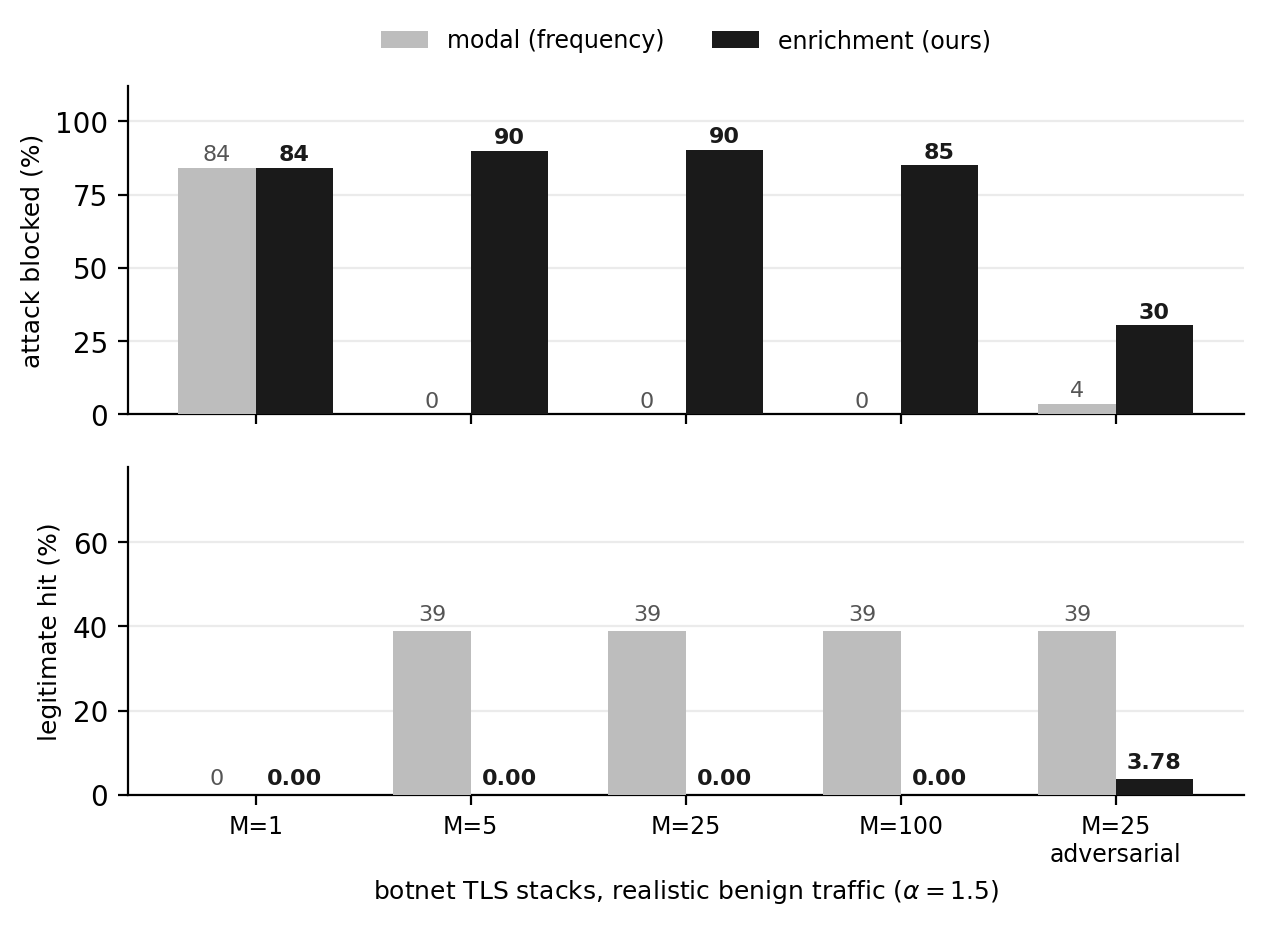
\includegraphics[width=\columnwidth]{figures/fig2_collateral.png}
\caption{Escolher o discriminador por frequência \emph{versus} por enriquecimento,
sob concentração realista de \emph{fingerprints} benignos ($\alpha = 1{,}5$). A
regra modal só se sustenta para \emph{botnet} monolítica; a partir de cinco
\emph{stacks} ela não bloqueia atacante algum e atinge $39\%$ dos usuários
legítimos. O enriquecimento é invariante à fragmentação e, sob adoção adversarial
de \emph{fingerprint}, recusa em vez de causar dano. $n = 15$ sementes.}
\label{fig:collateral}
\end{figure}

A mitigação só é significativa como par: o que o escopo derivado bloqueia, e
quanto custa. Reportamos ambos sobre $n = 15$ campanhas por configuração,
comparando a regra por frequência contra a regra por enriquecimento da
Seção~\ref{sec:evidence} (Fig.~\ref{fig:collateral}).

Para uma \emph{botnet} monolítica as duas concordam: $84{,}0\%$ das sessões
atacantes bloqueadas a $0{,}00\%$ de colateral, contra $100\%$ para um
\emph{rate-limit} global no \emph{endpoint}, que por definição desconecta todo
usuário legítimo do serviço atacado. Esse é o regime em que a regra por frequência
foi validada, e ele não é representativo. A partir de cinco \emph{stacks}, o
\emph{fingerprint} modal do \emph{cluster} passa a ser um \emph{legítimo} e a regra
inverte: $0{,}0\%$ do ataque bloqueado e $39{,}0\%$ do tráfego legítimo atingido.
Isso é pior do que não fazer nada, já que impõe o custo da mitigação e não entrega
nenhum de seus benefícios. Uma população benigna mais concentrada
($\alpha = 2{,}0$) eleva esse colateral para $61{,}1\%$.

O enriquecimento elimina a falha, bloqueando $90{,}0\%$, $90{,}3\%$ e $85{,}0\%$ do
ataque em $M = 5$, $25$ e $100$ \emph{stacks}, em todos os casos a
$\mathbf{0{,}00\%}$ de colateral, e reproduzindo a regra por frequência onde esta
funcionava. Os $10$--$15\%$ que sobrevivem são a cauda de atacantes com
\emph{fingerprints} avulsos: a mitigação de escopo derivado troca completude por
precisão.

\textbf{Duas condições delimitam o resultado.} A primeira é adversarial: quando a
\emph{botnet} adota \emph{fingerprints} benignos comuns, pouco fica enriquecido e a
regra bloqueia $30{,}4\%$ do ataque a $3{,}78\%$ de colateral, contra $3{,}6\%$ e
$39{,}0\%$ da regra por frequência. A vantagem cirúrgica é em larga medida
perdida, mas é perdida \emph{com segurança}: com um $\rho$ mais estrito o escopo
recusa nomear um \emph{fingerprint} e degenera para o controle global, que é o
relato correto quando não existe discriminador. A segunda é o perfil de fundo. Um
desvio moderado é tolerável (perfil com $\alpha = 2{,}0$ contra episódio com
$\alpha = 1{,}5$: $90{,}3\%$ de cobertura, $0{,}45\%$ de colateral); um perfil
plano ou ausente não é, pois então todo \emph{fingerprint} parece raro, a cabeça
benigna marca como enriquecida, e o colateral salta para $81{,}2\%$. A cobertura
não é afetada em nenhum dos casos, já que a qualidade do perfil governa a precisão
e não o \emph{recall}, de modo que mantê-lo é requisito de implantação e não
otimização.

\subsection{Custo e a Escolha de $W$}
\label{sec:latency}

O Apêndice~\ref{app:cost} mede as duas camadas do \emph{pipeline} em função da
ocupação da janela. Dois resultados importam: a admissão custa constantes
$14$--$19$~ns por par candidato, sustentando cerca de $84\,000$ admissões de sessão
por segundo em um núcleo com $|S_W| = 1\,000$; e a detecção é plana numa faixa de
$30\times$ em $W$, enquanto a ocupação do \emph{cluster}, e com ela o termo
quadrático de pares que $\Omega(S)$ implica, cresce $6{,}6\times$. Mantenha $W$ tão
pequeno quanto o tráfego permitir.

\subsection{Significância Estatística}

Aplicamos testes pareados de Wilcoxon sobre as $n = 30$ execuções, com correção de
Bonferroni e $d$ de Cohen. No regime distribuído ($K = 1000$), \textbf{(d)$-$(c)} é
significativa com $p_{\mathrm{Bonf}} = 7{,}5\times 10^{-9}$ e $d = 13{,}5$, e
\textbf{(d)$-$(a)} com $p_{\mathrm{Bonf}} = 7{,}5\times 10^{-9}$ e $d = 22{,}4$.
Tamanhos de efeito dessa magnitude refletem a natureza controlada do tráfego
sintético, que produz separação quase perfeita, e não devem ser lidos como
expectativa de desempenho em campo.

%% ====================================================================
\section{Discussão e Limitações}
\label{sec:discussion}

Cinco limitações delimitam a afirmação, intercaladas abaixo com dois parágrafos
que posicionam o arcabouço operacionalmente; outras estão no
Apêndice~\ref{app:limitations}.

\textbf{O ganho é específico de regime.} Contra ataques de origem única e alto
volume, limiares por IP ou por sessão têm desempenho comparável, e nos ataques
reais convencionais disponíveis em \emph{datasets} públicos um classificador por
sessão forte já alcança $\mathrm{AUC} \geq 0{,}98$, deixando ao raciocínio entre
sessões apenas um ganho marginal. A vantagem é decisiva apenas quando a campanha é
distribuída \emph{e} furtiva. Este trabalho não substitui defesas volumétricas; as
complementa. Validar a abordagem sobre tráfego furtivo distribuído
\emph{capturado}, que nenhum \emph{benchmark} público oferece, é a direção
experimental mais importante.

\textbf{A avaliação sintética demonstra um mecanismo, não desempenho em campo.} No
cenário sintético, os sinais de coordenação presentes na campanha são exatamente
aqueles medidos pela configuração (d), e as sessões atacantes tomam seus atributos
por sessão de distribuições benignas reais. A não-separabilidade por sessão da
Tabela~\ref{tab:ablation} não é, portanto, artefato de um \emph{baseline}
enfraquecido, já que quatro famílias de modelo com todos os atributos de fluxo
permanecem no acaso. O mimetismo é imposto por construção, de modo que o resultado
mostra o mecanismo sob a hipótese de indistinguibilidade por sessão perfeita, e não prova
desempenho sobre uma captura real desse regime.

\textbf{Detecção e derivação de escopo dependem ambas de um discriminador de peso
alto observável.} Uma varredura de robustez ($n = 10$) torna a dependência
explícita: à medida que a fração de origens que compartilham o \emph{fingerprint}
TLS cai, a $\mathrm{AUC}$(d) decresce monotonicamente de $1{,}00$ para
$\approx 0{,}74$ sob randomização total. Esse resíduo acima do acaso é artefato de
um \emph{pool} finito de JA4 benigno, de modo que sob diversidade em escala de
internet ele deve tender ao acaso. A convergência de \emph{endpoint} \emph{não}
compensa a perda do JA4 quando os usuários legítimos compartilham o
\emph{endpoint}, porque eles também convergem nele. Adversários podem forjar o JA4
com ferramentas como \texttt{curl-impersonate}, aplicar \emph{jitter} à
temporização e rotacionar identidades; a família ponderada tolera quebra parcial,
já que os sinais de peso alto remanescentes carregam o \emph{cluster}, mas quebrar
três ou mais de uma vez a degrada em direção ao acaso. A adoção ampla do Encrypted
Client Hello~\cite{ietf2024ech} poderia igualmente tornar o JA4 inobservável,
exigindo metadados TLS alternativos para compensar.

\textbf{Posicionamento operacional.} O arcabouço fecha um laço de gestão em vez de
emitir rótulos: detecção, evidência e escopo saem de uma passagem sobre o mesmo
grafo, de modo que o que chega ao operador ou a um \emph{playbook} de SOAR é um
\emph{course-of-action} STIX já parametrizado pelo discriminador que justificou o
veredicto. A janela deslizante é o que torna isso viável (Seção~\ref{sec:latency}).
É um complemento no plano de sessão às defesas volumétricas na borda, não um
substituto.

\textbf{Paralelismo e particionamento.} A própria regra dita a chave natural de
partição. A condição (ii) exige que toda sessão de $S$ tenha o mesmo
\emph{endpoint} $e$ como alvo, então particionar a janela ativa por
\emph{endpoint} avalia \texttt{CoordinatedHTTPFlood} \emph{exatamente}, sem tráfego
entre partições: o detector torna-se trivialmente paralelo sobre \emph{endpoints},
e como a janela limita $|S_W|$, o estado por partição não cresce com o volume
acumulado de tráfego. O custo não é zero, contudo. Particionar por \emph{endpoint}
esconde uma campanha que espalha um mesmo JA4 por muitos \emph{endpoints}, já que
nenhuma partição acumula pares coordenados suficientes para ultrapassar
$\tau_{\mathrm{cluster}}$; particionar por JA4 preserva exatamente essas campanhas
e quebra a condição de \emph{endpoint}. Nenhuma chave isolada preserva as seis
sub-relações, e isso é propriedade de $\Omega(S)$ e não de qualquer implementação.
O desenho que isso sugere, não implementado, é em dois níveis: trabalhadores
particionados por \emph{endpoint} mais um \emph{sketch} global sobre
identificadores de peso alto para recuperar campanhas entre \emph{endpoints};
quantificar o \emph{recall} perdido pelo primeiro nível e recuperado pelo segundo é
pré-requisito para implantação em escala de CDN. Tomadas em conjunto com a
Seção~\ref{sec:latency}, essas observações compõem um único argumento de
escalabilidade: o particionamento por \emph{endpoint} é exato e dispensa
coordenação, um $W$ pequeno não custa detecção enquanto corta o termo quadrático de
pares, e a admissão custa microssegundos. Numa implantação corretamente
configurada, o termo quadrático portanto nunca morde.

\textbf{A ablação mede representação, não formalismo.} A configuração (d) alcança a
evidência do grafo por atributos e não por SPARQL: um modelo linear sobre os mesmos
três atributos entre sessões ainda alcança $0{,}799$ contra $0{,}495$ do conjunto
por sessão, de modo que o ganho de AUC na Tabela~\ref{tab:ablation} é atribuível a
representar estrutura entre sessões, e não a expressá-la em OWL. A camada simbólica
é evidenciada à parte, pela Tabela~\ref{tab:symbolic}, e apenas em parte: ela não
supera o modelo aprendido contra \emph{botnet} monolítica, e sua vantagem aparece
quando a fragmentação ou a adoção adversarial de \emph{fingerprint} tornam a
distribuição de escores inutilizável para um limiar de falso positivo zero. As duas
afirmações devem ser lidas separadamente.

\textbf{Cobertura de família de ataque, protocolo e \emph{dataset}.} A ontologia e
a avaliação cobrem a família Slow HTTP DoS sobre HTTP/1.1; ataques sobre HTTP/2 e
outros protocolos de aplicação exigem sub-relações que não modelamos. A validação
em dados reais abrange seis ataques (Slowloris, Slowhttptest, HULK, GoldenEye,
HTTP-Flood, DoS-Other) em dois \emph{datasets}, mas todos são capturas de
\emph{testbed} de laboratório, e a comparação direta com o KLAGE é necessariamente
de ataque único, já que é isso que o KLAGE publica. Essa comparação difere também
em granularidade e protocolo, de modo que reproduzir o KLAGE sob nosso protocolo é
necessário antes de qualquer afirmação de superioridade.

%% ====================================================================
\section{Conclusão}
\label{sec:conclusion}

Modelamos a sessão HTTP como entidade ontológica de primeira classe e substituímos
a relação plana entre sessões por seis sub-propriedades tipadas, ponderadas pelo
custo que o atacante teria para quebrar cada sinal. Uma regra SPARQL/SWRL dispara
sobre a massa ponderada dessas sub-relações, de modo que uma única derivação serve
ao mesmo tempo como veredicto, cadeia de evidência e escopo da mitigação.

Contra campanhas furtivas distribuídas, a detecção por sessão fica no acaso em
quatro famílias de modelo, mesmo com o conjunto completo de atributos de fluxo,
enquanto o arcabouço detecta de forma consistente ($0{,}50$ \emph{vs.}\ $0{,}98$ de
ROC AUC; $d = 22{,}4$); em ataques reais convencionais o ganho é marginal, porque
um classificador por sessão forte já basta. Do lado da mitigação, o estudo produziu
um resultado negativo que vale tanto quanto o positivo: derivar o escopo pela
propriedade que a maioria do \emph{cluster} compartilha seleciona um
\emph{fingerprint} legítimo assim que a \emph{botnet} abrange mais de um
\emph{stack} TLS, bloqueando usuários em vez de atacantes. O enriquecimento sobre
um perfil de tráfego normal restaura $85$--$90\%$ de cobertura a $0{,}00\%$ de
colateral. E, medido como detector, esse caminho simbólico recupera $90\%$ de uma
campanha de 25 \emph{stacks} onde o modelo aprendido recupera $36\%$ no mesmo ponto
de operação de falso positivo zero. Essa lacuna é escondida pela AUC, e é a
evidência mais clara de que o grafo se paga. Direções imediatas são os ataques
sobre HTTP/2 e uma campanha furtiva capturada, que nenhum \emph{benchmark} ainda
oferece.

\section*{Agradecimento}
Agradecemos à Azion Technologies por autorizar a medição agregada de
\emph{fingerprints} reportada na Seção~\ref{sec:method}.

\bibliographystyle{IEEEtran}
\bibliography{references}

%% ====================================================================
\appendices

\section{Instanciação das Sub-Relações \texttt{relatedBy}}
\label{app:algorithms}

Para cada par $(s_a,s_b)$ de sessões ativas em $W$, os procedimentos de decisão a
seguir determinam se a aresta correspondente é instanciada.

\textbf{\texttt{TLSFingerprint}.} Casamento em duas etapas: igualdade exata do JA4
completo ou, na falta dela, variantes próximas (mesmo prefixo de
transporte/versão TLS/ALPN, com no máximo um símbolo de diferença nos blocos
ordenados de \emph{cipher} ou de extensões), instanciada com anotação
\emph{ja4\_distance = 1}. Isso absorve a variação entre versões de uma mesma
biblioteca cliente sem admitir casamentos espúrios entre \emph{stacks} distintos.
Custo $O(1)$ por par.

\textbf{\texttt{ReusedIdentity}.} Instanciada em qualquer sobreposição não-vazia
entre os conjuntos de identidades observadas,
$(\mathrm{cookie}(s_a) \cap \mathrm{cookie}(s_b)) \cup (\mathrm{token}(s_a) \cap
\mathrm{token}(s_b)) \cup (\mathrm{user}(s_a) \cap \mathrm{user}(s_b)) \neq
\emptyset$. JWTs são decodificados e comparados pelo \emph{claim} \texttt{sub};
\emph{cookies} e \emph{usernames} são normalizados (\emph{trim}, caixa baixa).
Custo $O(1)$ amortizado com índice invertido.

\textbf{\texttt{TemporalPattern}.} Com $\Delta(s)$ a sequência de intervalos entre
chegadas, computamos
$d_{\mathrm{DTW}}(s_a,s_b) = \mathrm{DTW}(\Delta(s_a),\Delta(s_b)) /
\max(|\Delta(s_a)|,|\Delta(s_b)|)$ e instanciamos quando
$d_{\mathrm{DTW}} \leq \tau_{\mathrm{DTW}}$. Sessões com menos de três requisições
são puladas. O FastDTW sob banda de Sakoe--Chiba de largura constante reduz o custo
por par de $O(n^2)$ para $O(n)$, e \emph{locality-sensitive hashing} sobre vetores
de resumo ($\bar\delta$, $\sigma_\delta$, $\delta_{\min}$, $\delta_{\max}$,
entropia) evita a comparação de todos os pares.

\textbf{\texttt{PayloadSignature}.} Com
$\mathbf{p}(s) = (\overline{\mathrm{len}}, \sigma_{\mathrm{len}}, h_{\mathrm{UA}},
h_{\mathrm{CT}})$, isto é, média e desvio-padrão do tamanho do corpo mais
\emph{hashes} do User-Agent e do Content-Type predominantes, a aresta é
instanciada quando a similaridade de cosseno excede $\tau_{\mathrm{payload}}$.
Custo $O(1)$ dados os vetores pré-computados.

\textbf{\texttt{EndpointConvergence}.} Instanciada quando ambas as sessões
convergem no mesmo \emph{endpoint}, sob normalização de padrão de caminho
(\texttt{/api/users/12345} $\rightarrow$ \texttt{/api/users/\{id\}}) por padrão; um
casamento adicional de caminho exato anota a aresta com \emph{exact = true}. Custo
$O(1)$ com índice em árvore de prefixos.

\textbf{\texttt{NetworkProximity}.} Instanciada num prefixo IPv4 /24 (ou IPv6 /48)
compartilhado, ou num ASN compartilhado, ou em ambos; quando ambos valem, a aresta
é anotada com \emph{strong = true}. A resolução de ASN usa tabelas BGP atuais.
Custo $O(1)$ com índice invertido de prefixo.

\begin{listing}[t]
\footnotesize
\hrule\vspace{2pt}
\begin{verbatim}
# SWRL (Horn): instancia uma sub-relacao
ApplicationSession(?a) ^ ApplicationSession(?b) ^
  differentFrom(?a,?b) ^
  tlsJa4(?a,?j) ^ tlsJa4(?b,?j)
  -> relatedByTLSFingerprint(?a,?b)

# SPARQL: agregacao ponderada sobre o cluster
SELECT ?e (SUM(?w) AS ?omega) (COUNT(*) AS ?pairs)
WHERE { ?a kg:targets ?e . ?b kg:targets ?e .
        ?a ?rel ?b .
        ?rel rdfs:subPropertyOf kg:relatedTo ;
             kg:coordinationWeight ?w .
        FILTER(STR(?a) < STR(?b)) }
GROUP BY ?e HAVING (SUM(?w) >= ?tau)
\end{verbatim}
\vspace{-4pt}\hrule
\caption{Veredicto como derivação: regras de Horn materializam as arestas tipadas
entre sessões; uma agregação SPARQL aplica os pesos declarados na ontologia e
dispara a regra. Os \emph{bindings} que satisfazem a consulta \emph{são} a cadeia
de evidência.}
\label{lst:rules}
\end{listing}

\section{Calibração dos Pesos}
\label{app:calibration}

A calibração empírica depende criticamente do realismo do tráfego. Em
\emph{datasets} de laboratório, com poucas dezenas de \emph{fingerprints} JA4
distintos, a otimização chega a inverter o sinal do TLS, porque as sessões
benignas compartilham \emph{fingerprints} mais do que as campanhas parcialmente
coordenadas; isso é artefato de \emph{testbed} pela baixa diversidade de JA4,
ausente na internet real.

No cenário realista (milhares de \emph{fingerprints} JA4 legítimos, com usuários
acessando o serviço atacado), calibramos maximizando a ROC AUC por sessão de
ataque \emph{vs.}\ benigno sobre o escore
$w_{\mathrm{tls}}\,z(\mathrm{ja4}) + w_{\mathrm{ep}}\,z(\mathrm{conv.\ endpoint})
+ w_{\mathrm{net}}\,z(\mathrm{prox.\ rede})$ com atributos padronizados, sobre o
\emph{grid} $\{0{,}3\ldots1{,}0\}^3$ (125 combinações, 60 cenários, 91\,500
sessões). O resultado corrobora a ordenação proposta: o melhor vetor é
$(w_{\mathrm{tls}}{=}1{,}0,\ w_{\mathrm{ep}}{=}0{,}3,\ w_{\mathrm{net}}{=}0{,}3)$,
e o \emph{fingerprint} TLS é o único sinal individualmente discriminativo
($\mathrm{AUC}$ isolada $= 0{,}93$, contra $0{,}50$ da convergência de
\emph{endpoint} e $0{,}58$ da proximidade de rede). Os pesos da
Fig.~\ref{fig:ontology} $(1{,}0,\ 0{,}6,\ 0{,}3)$ atingem a mesma
$\mathrm{AUC}$ ótima $= 0{,}943$ e são insensíveis a perturbação de $\pm20\%$ (sem
queda mensurável). A calibração valida portanto a \emph{ordenação}; no regime puro
de mesmo serviço, os pesos médio e baixo não são separadamente identificáveis, já
que isoladamente ambos ficam perto do acaso, e seus valores absolutos permanecem em
aberto até que haja tráfego de produção com sinais parciais e conflitantes.

\section{Limitações Adicionais}
\label{app:limitations}

\textbf{Instrumentação de sessão e identidade.} A abordagem assume que sessões,
identidades e \emph{fingerprints} TLS podem ser extraídos dos eventos de tráfego;
onde essa instrumentação for parcial ou ruidosa, o desempenho degrada.

\textbf{Custo de manutenção do grafo.} Os números da camada simbólica do
Apêndice~\ref{app:cost} vêm de uma implementação de referência em memória com
\texttt{rdflib}, e não do \emph{backend} Jena/TDB2, de modo que são um limite
superior; e escalar para tráfego em escala de CDN requer o particionamento
horizontal discutido na Seção~\ref{sec:discussion}, que não implementamos.

\textbf{Cobertura de protocolo.} A ontologia atual cobre a família Slow HTTP DoS
sobre HTTP/1.1. Ataques sobre HTTP/2 e outros protocolos de
aplicação (DNS, gRPC) exigem sub-relações adicionais.

\textbf{Amplitude de \emph{datasets}.} A validação em dados reais cobre um
\emph{dataset} e um ataque para a comparação direta, mais seis ataques entre
CICIDS2017 e CIC-IoT2023 para a análise de regime. RT-IoT2022, CIC-DDoS2019 e
tráfego de produção anonimizado ficam como trabalho futuro.

\textbf{Validação da explicação.} As cadeias de evidência foram avaliadas quanto a
completude estrutural e acionabilidade ($7/7$), mas a acionabilidade
\emph{percebida}, isto é, um estudo com analistas humanos medindo tempo até a
decisão e compreensão, não foi conduzida.

\begin{figure}[h]
\centering
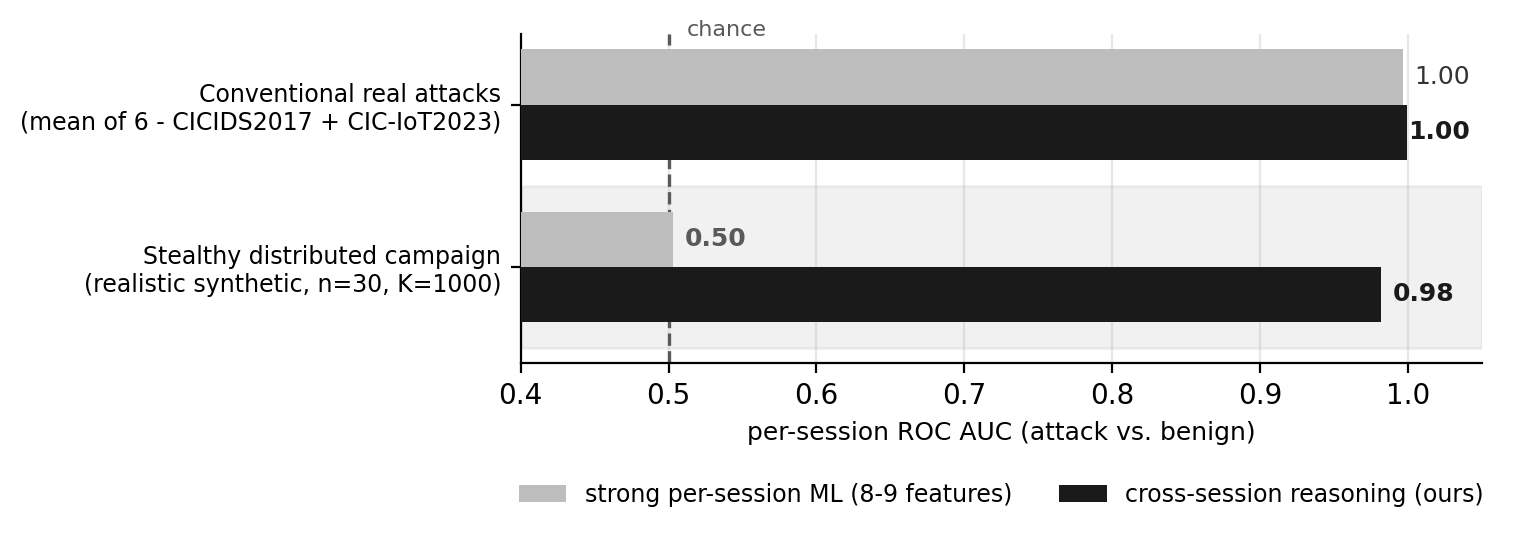
\includegraphics[width=\columnwidth]{figures/fig3_regime.png}
\caption{Onde o raciocínio entre sessões é \emph{necessário}. Em ataques reais
convencionais um classificador por sessão forte já satura; só no regime furtivo
distribuído a detecção por sessão colapsa para o acaso enquanto o raciocínio entre
sessões se sustenta.}
\label{fig:regime}
\end{figure}

\section{Modelo de Custo e Sensibilidade à Janela}
\label{app:cost}

\begin{figure}[h]
\centering
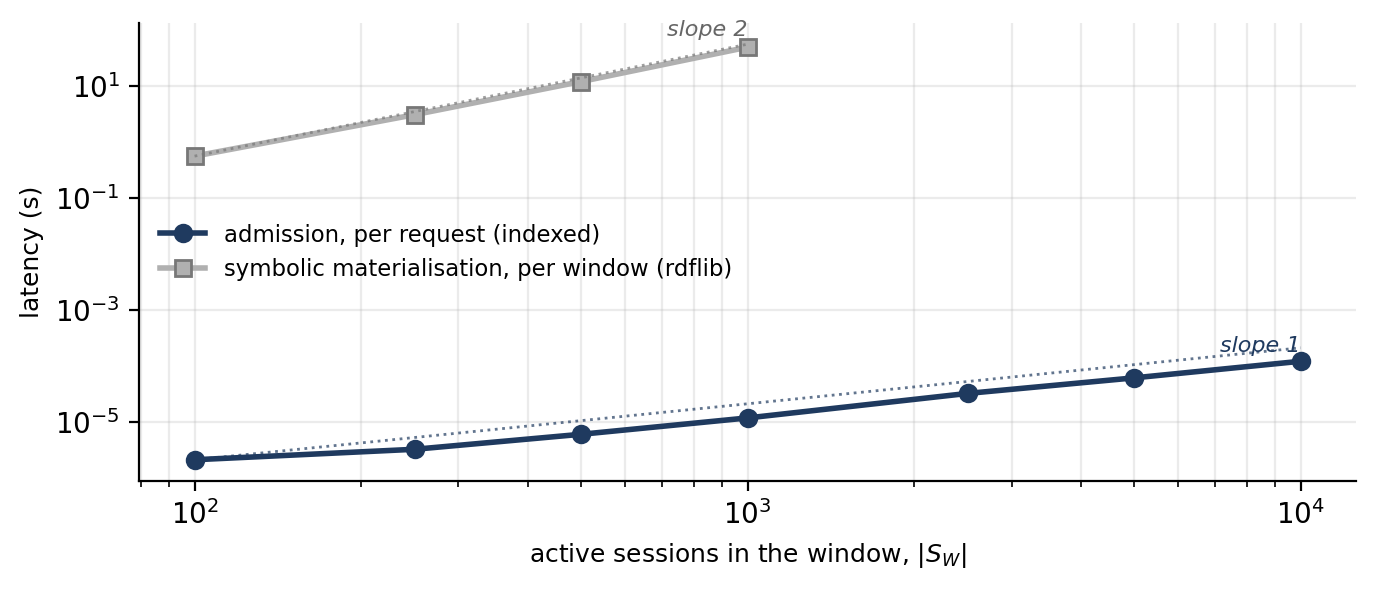
\includegraphics[width=\columnwidth]{figures/fig4_latency.png}
\caption{Custo das duas camadas em função da ocupação da janela. A admissão por
requisição é linear em $|S_W|$ e permanece na faixa de microssegundos; a
materialização simbólica por janela é linear no número de arestas RDF, que por sua
vez é quadrático em $|S_W|$. Retas de referência ancoradas no primeiro ponto de
cada série.}
\label{fig:latency}
\end{figure}

As duas camadas operam em taxas diferentes, já que a admissão acontece por
requisição e a materialização simbólica com a agregação de $\Omega$ acontece por
janela, então as medimos separadamente, sobre uma janela sintética na mistura
realista de mesmo serviço (30\% das sessões numa campanha compartilhando um JA4 de
\emph{botnet}, JA4 benigno de um \emph{pool} de 2\,000, oito \emph{endpoints}, /24s
dispersos); medianas sobre três repetições em um núcleo. Este é um modelo de custo
do algoritmo como especificado, e não um \emph{benchmark} de sistema: o caminho de
admissão é implementação direta do esquema de índices invertidos da
Seção~\ref{sec:pipeline}, e a camada simbólica roda sobre uma implementação de
referência em memória com \texttt{rdflib}, e não sobre o \emph{backend} Jena/TDB2
usado no \emph{pipeline} de \emph{datasets}, de modo que seus números são um limite
superior.

A admissão se comporta como o limite prevê (Fig.~\ref{fig:latency}): a latência
mediana cresce de $2{,}1\,\mu$s em $|S_W| = 100$ para $122\,\mu$s em
$|S_W| = 10\,000$, acompanhando a contagem de pares candidatos (148 a 6\,495
arestas por admissão) a constantes $14$--$19$~ns por par.

A camada simbólica é ordens de magnitude mais cara: $0{,}56$~s em $|S_W| = 100$,
subindo para $49{,}7$~s em $|S_W| = 1\,000$. Lida por unidade de trabalho, contudo,
o custo permanece constante em $\approx 187\,\mu$s por aresta RDF materializada em
todos os tamanhos, de modo que a camada é \emph{linear em arestas}; é a contagem de
arestas que cresce quadraticamente, porque $\Omega(S)$ é definida sobre pares. O
termo quadrático é portanto propriedade da regra, e não do \emph{backend}, e aponta
para a divisão de implantação que a arquitetura já sugere: detectar pelo caminho
indexado de admissão, e materializar RDF apenas para os \emph{clusters} que
disparam, isto é, o subconjunto da cadeia de evidência e não a janela inteira.

\begin{table}[h]
\centering
\caption{Varredura da janela, $K = 1000$, $n = 10$ sementes. A detecção é plana
numa faixa de $30\times$ em $W$, enquanto a ocupação do \emph{cluster}, e portanto
o termo quadrático de pares, cresce com ela.}
\label{tab:window}
\footnotesize
\setlength{\tabcolsep}{4pt}
\begin{tabular}{@{}rrrcccc@{}}
\toprule
$W$ (s) & \emph{clusters} & $|S|$ médio & (a) & (b) & (c) & (d) \\
\midrule
   60 & 16 & 132 & 0,505 & 0,508 & 0,664 & 0,976 \\
  120 & 11 & 207 & 0,505 & 0,508 & 0,663 & 0,977 \\
  300 &  6 & 364 & 0,505 & 0,508 & 0,664 & 0,977 \\
  600 &  4 & 557 & 0,505 & 0,508 & 0,664 & 0,978 \\
 1800 &  3 & 867 & 0,505 & 0,508 & 0,664 & 0,978 \\
\bottomrule
\end{tabular}
\end{table}

$W$ entra apenas na atribuição de \emph{clusters} de detecção, então a varredura
recomputa os atributos entre sessões sobre os mesmos cenários em cache. A
Tabela~\ref{tab:window} mostra que a detecção é insensível a ele entre $60$ e
$1800$~s: o atributo discriminativo é a fração de um \emph{cluster} que compartilha
um mesmo JA4, uma razão que não muda conforme o \emph{cluster} cresce, ao passo que
o tamanho do \emph{cluster} sozinho carrega pouco, e é por isso que (c) fica em
$0{,}664$ o tempo todo. Dois limites desse resultado: os cenários têm um único
\emph{endpoint} alvo, então $W$ é o único botão de agrupamento e uma implantação
multi-\emph{endpoint} com campanhas interleaved pode se comportar de outra forma; e
$W$ ainda precisa ser longo o bastante para que um \emph{cluster} se forme, o que
em $W = 60$~s já significa $\approx 132$ sessões aqui.

\begin{listing}[t]
\footnotesize
\hrule\vspace{2pt}
\begin{verbatim}
"@type": "kg:CoordinatedHTTPFlood",
"kg:clusterSize": 6, "kg:coordinationScore": 10.8,
"kg:activatedSubRelations": [
 {"@type": "kg:relatedByEndpointConvergence",
  "kg:coordinationWeight": 0.6, "kg:linkedPairs": 15,
  "kg:weightedContribution": 9.0},
 {"@type": "kg:relatedByNetworkProximity",
  "kg:coordinationWeight": 0.3, "kg:linkedPairs": 6,
  "kg:weightedContribution": 1.8}],
"kg:derivedMitigationScope": {
  "kg:endpoint": "192.168.10.50:80",
  "kg:srcNet24":  "172.16.0.0/24"}
\end{verbatim}
\vspace{-4pt}\hrule
\caption{Cadeia de evidência emitida para o \emph{cluster} DoS-Other do CICIDS2017
(JSON-LD, abreviada). Cada termo de $\Omega(S) = 10{,}8$ é atribuível a uma
sub-relação, uma contagem de pares e um peso, e o último campo é o filtro
efetivamente aplicado. A exportação STIX~2.1 carrega o mesmo conteúdo como padrão
de \emph{indicator} mais um \emph{course-of-action} ligado por \emph{mitigates}.}
\label{lst:chain}
\end{listing}

\section{Reprodutibilidade}
\label{app:repro}

A implementação de referência está disponível em
\url{https://github.com/Natanael0liveira/knowledge-graph-ddos-article} sob licença
permissiva, organizada por etapa experimental: o \emph{pipeline} de extração
(PCAP $\rightarrow$ JA4 e fluxos $\rightarrow$ sessões $\rightarrow$ grafo); o
gerador sintético calibrado, incluindo os três parâmetros de realismo da
Seção~\ref{sec:method}, isto é, expoente de Zipf da popularidade de
\emph{fingerprints} benignos, número de \emph{stacks} TLS da \emph{botnet} e adoção
adversarial de \emph{fingerprints} benignos comuns, com as configurações de cenário
canônico e adversarial; a ablação, os \emph{baselines} acadêmicos e as quatro
famílias de modelo; o executor estatístico; a comparação contra o estado da arte
publicado; a camada simbólica (regras SWRL mais a agregação SPARQL, com pesos lidos
da ontologia); e os módulos de evidência e mitigação.

As duas derivações de escopo são distribuídas lado a lado, deliberadamente: a regra
por frequência que falha e a regra por enriquecimento que a substitui, de modo que
o resultado negativo da Seção~\ref{sec:collateral} seja reprodutível e não apenas
afirmado. O perfil de fundo de que o teste de enriquecimento precisa é produzido
por uma execução do gerador sem ataque, então nenhum rótulo entra no caminho de
decisão em momento algum. O modelo de custo do Apêndice~\ref{app:cost} não requer
\emph{dataset} algum e roda em qualquer lugar.

As sementes são fixas, a orquestração é feita por Makefiles, e os artefatos, isto é
figuras, distribuições calibradas e resultados agregados, são versionados; cada
tabela e cada figura de dados deste artigo é regenerada por um único comando por
etapa. A Fig.~\ref{fig:ontology} é um esquema desenhado à mão, cuja fonte editável
acompanha o artefato. A
ontologia OWL é fornecida em RDF/XML, com cada sub-propriedade \texttt{relatedBy}
anotada com seu \texttt{coordinationWeight}. Pretendemos submeter esses artefatos à
trilha de Artifact Evaluation.

\end{document}
